\section{Macarons}
The two meringue based halves are made from almonds, egg white, and sugar. The filling is usually a ganache or buttercream.

\begin{figure}[!htb]
    \begin{center}
    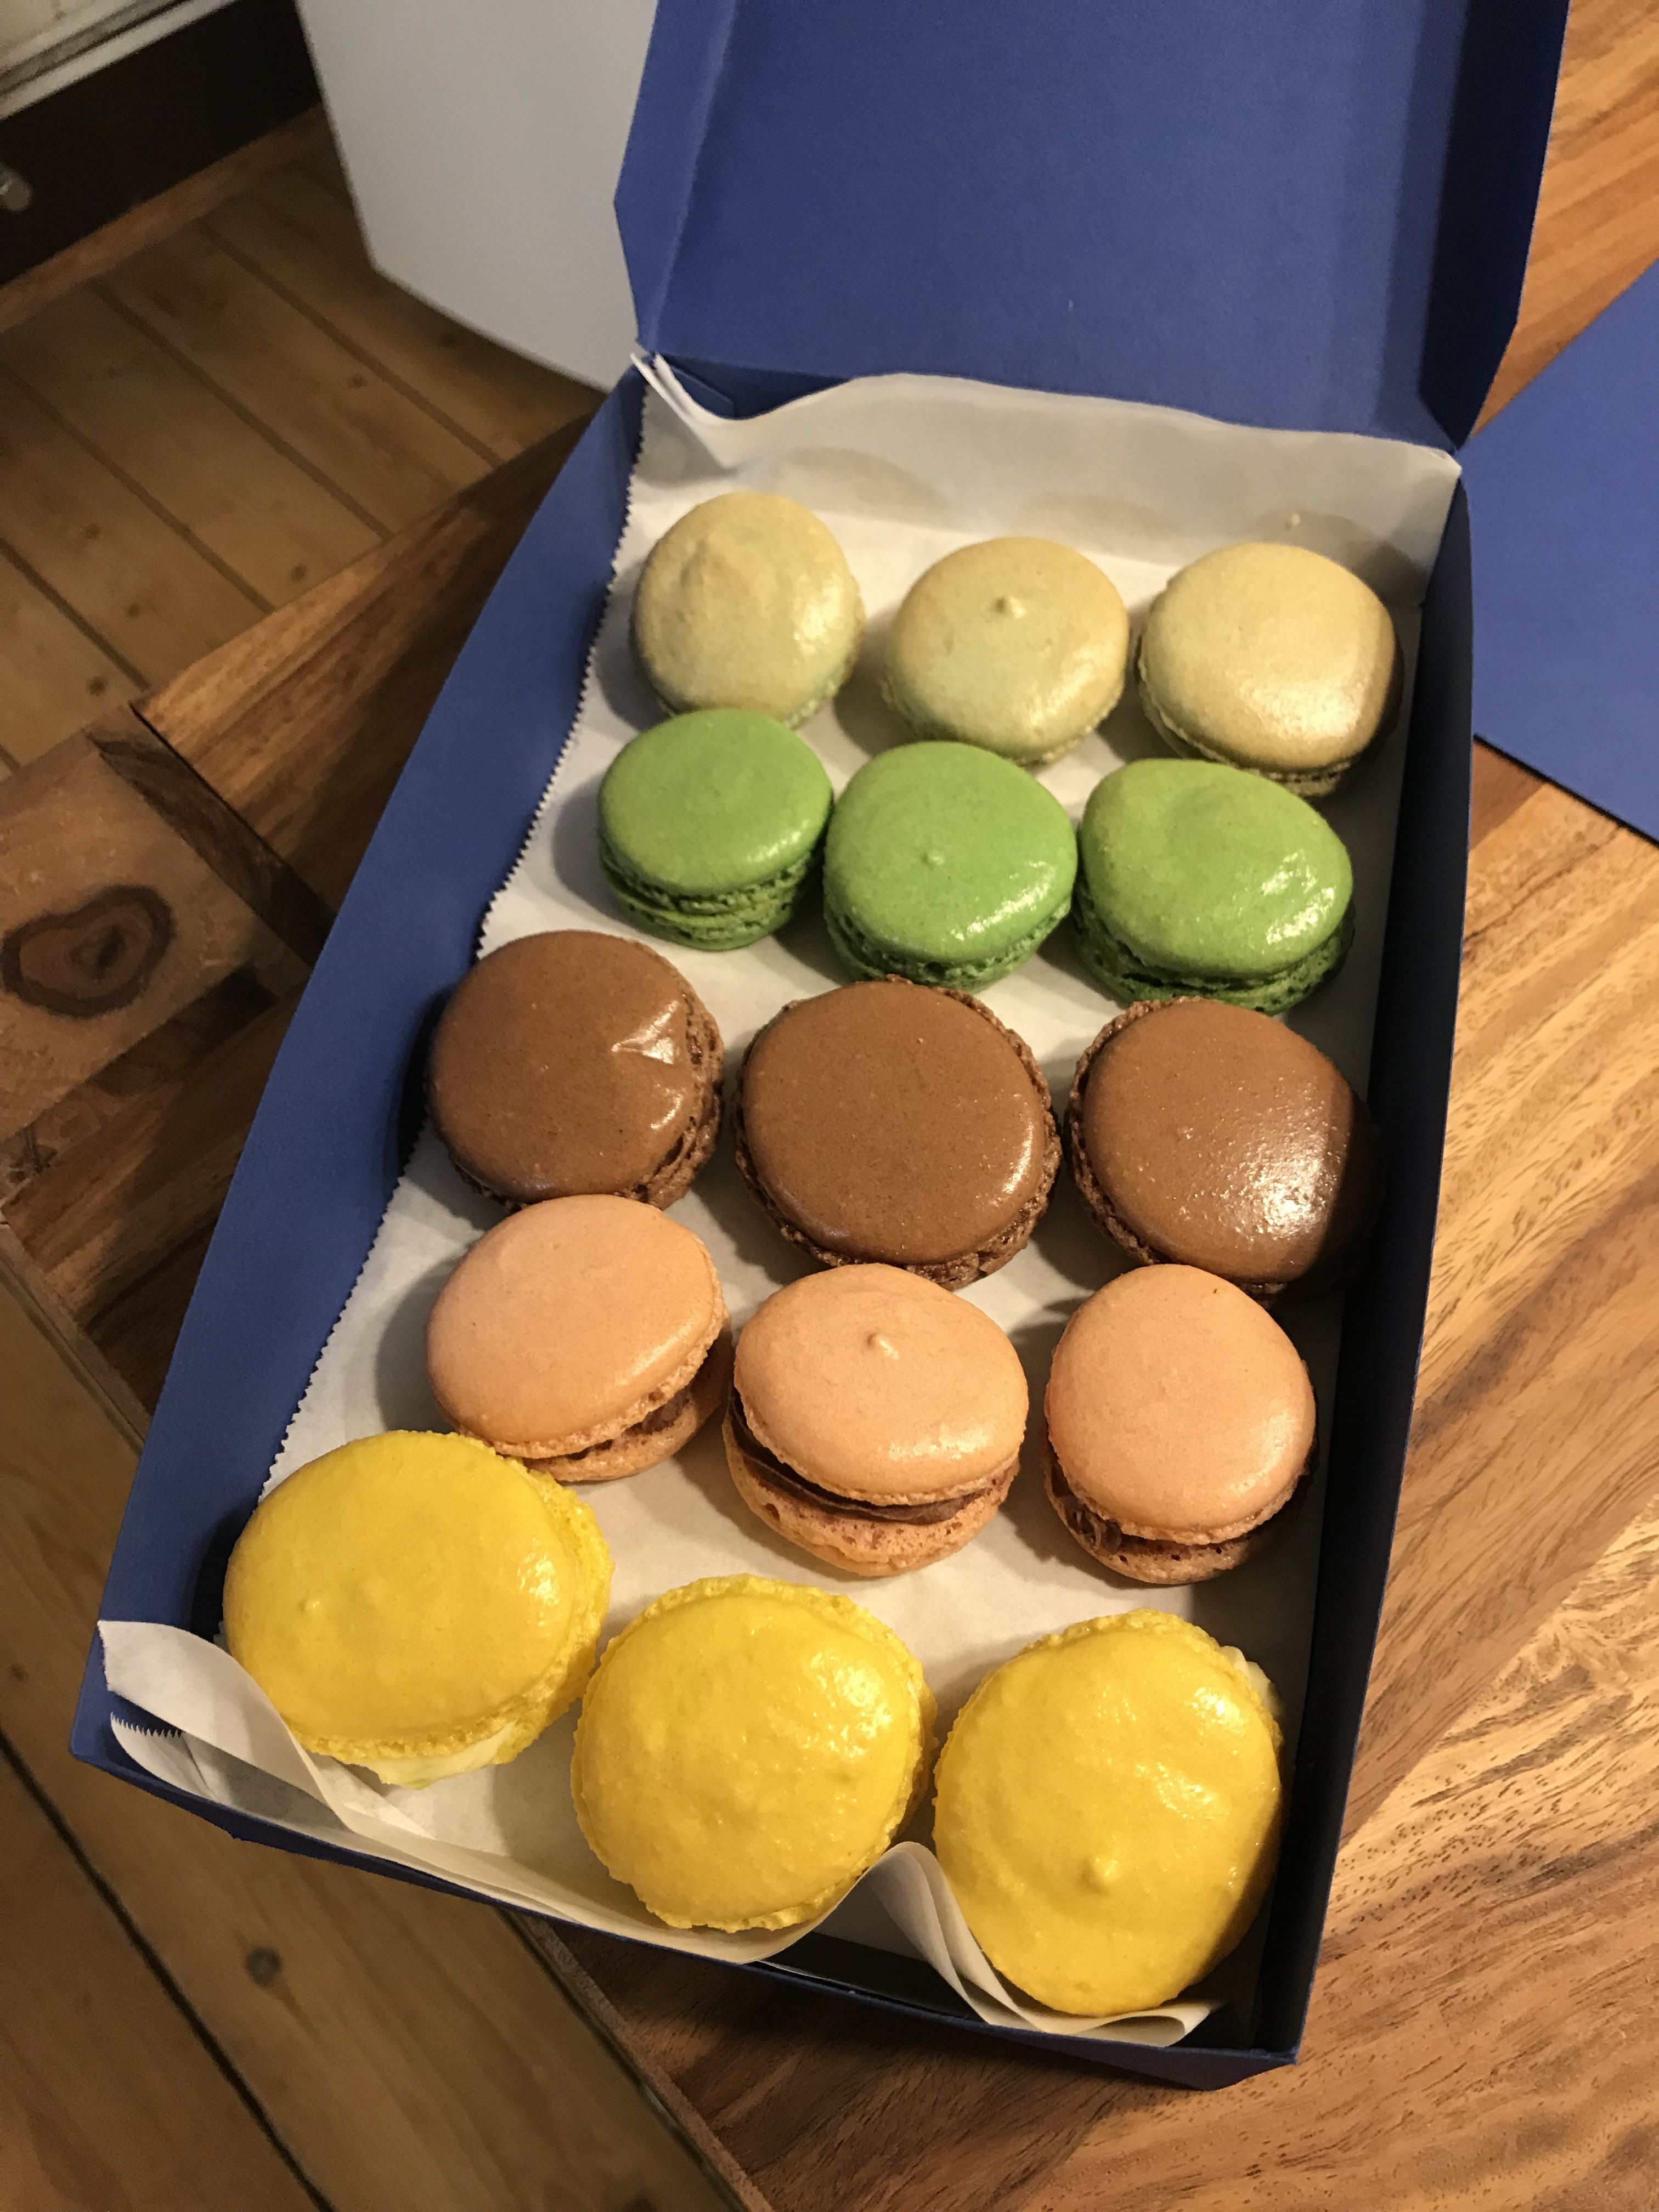
\includegraphics[width=6cm]{Pictures/Desserts/macarons_1.jpg}
    \caption[Macarons]{Macarons}
    \label{fig:macarons}
    \end{center}
\end{figure}
\subsection*{Ingredients}
\begin{tabular}{ l l }
  36g & egg white \\
  45g & ground almonds \\
  75g & powdered sugar \\
  10g & sugar \\
\end{tabular}

\subsection*{Description}
\begin{enumerate}
	\item Mix the powdered sugar and ground almonds and sift them to get a homogeneous mix without any large chunks.
	\item Whisk the egg white. In the end, slowly add the sugar while continuing to whisk. Optional: add food coloring
	\item Fold the almond-sugar mix in: add 1/3 of the mix to the egg white and carefully fold it in, add the next third and so on.
	\item Fill the mix into a small freeze bag or other plastic bag and cut off one corner.
	\item Form small (3-4cm diameter) circles on a tray with baking paper.
	\item Lightly tap the baking tray from underneath to allow air bubbles trapped in the dough to escape. This leads to a nicer round shape and a more even surface.
	\item preheat the oven to 145 deg. Celsius
	\item Let the macarons sit a room temperature for 20-30 minutes.
	\item Bake for 10-12 minutes
\end{enumerate}

